\documentclass{article}
\usepackage[utf8]{inputenc}
\usepackage[french]{babel}
\usepackage{amsmath}
\usepackage{listings}
\usepackage{hyperref}
\usepackage{xcolor}
\usepackage{graphicx}
\usepackage[style=authoryear]{biblatex}
\usepackage{fancyhdr}
\usepackage{braket}
\usepackage{float}
\usepackage{color}
\usepackage{tabularx}

\definecolor{codegreen}{rgb}{0,0.6,0}
\definecolor{codegray}{rgb}{0.5,0.5,0.5}
\definecolor{codepurple}{rgb}{0.58,0,0.82}
\definecolor{backcolour}{rgb}{0.95,0.95,0.92}

\lstdefinestyle{mystyle}{
  backgroundcolor=\color{backcolour},   
  commentstyle=\color{codegreen},
  keywordstyle=\color{magenta},
  numberstyle=\tiny\color{codegray},
  stringstyle=\color{codepurple},
  basicstyle=\ttfamily\footnotesize,
  breakatwhitespace=false,         
  breaklines=true,                 
  captionpos=b,                    
  keepspaces=true,                 
  numbers=left,                    
  numbersep=5pt,                  
  showspaces=false,                
  showstringspaces=false,
  showtabs=false,                  
  tabsize=2
}

\pagestyle{fancy}

\fancyhf{}
\fancyhead[L]{Rapport de séminaire : L'algorithme quantique}
\fancyhead[R]{RAETH et SANNA, L3STI}
\fancyfoot[C]{Page n°\thepage}

\addbibresource{ref.bib}

\title{Rapport de séminaire :\\L'algorithme quantique}
\author{Léandre RAETH, Thomas SANNA\\L3 Sciences et Technologies, Parcours Informatique}
\date{\today}

\begin{document}

\begin{titlepage}
  \begin{center}
      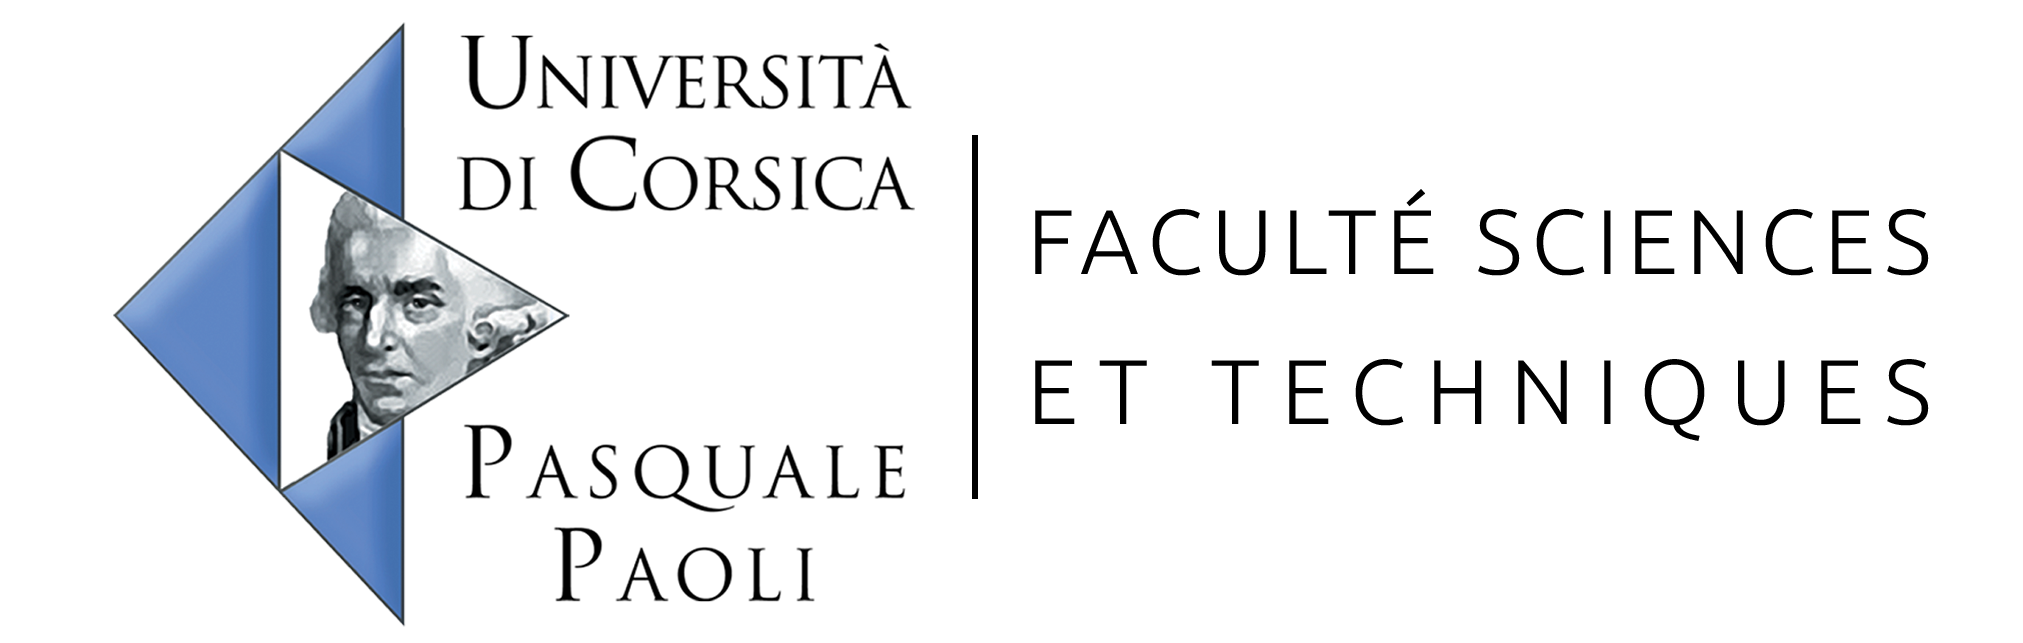
\includegraphics[width=0.5\textwidth]{img/univCorse.png}\\[1cm]
      
      \textsc{\LARGE Université de Corse}\\[1.5cm]
      
      \textsc{\Large Année universitaire 2024-2025}\\[0.5cm]
      
      \vfill
      
      \hrulefill\\[0.4cm]
      {\Huge \bfseries Rapport de Séminaire}\\[0.4cm]
      \hrulefill\\[1.5cm]
      
      \textsc{\Large L'algorithme quantique}\\[0.5cm]
      
      \vfill
      
      \textbf{Présenté par :}\\
      Léandre RAETH, Thomas SANNA\\
      
      \vfill
      
      \textbf{Séminaire présenté le 03/04/2025}\\
      \vfill
      
      \textsc{L3 Sciences et Technologies, Parcours Informatique}
      
  \end{center}
\end{titlepage}

\break\begin{abstract}
  Ce rapport de séminaire vise à vulgariser le sujet de l'algorithme quantique pour un public non-initié. Nous expliquons les concepts fondamentaux de l'informatique quantique, en mettant l'accent sur la génération de nombres aléatoires, et présentons un exemple de code utilisant le framework Qiskit. Nous discutons également des défis actuels et des perspectives futures de l'informatique quantique.
\end{abstract}

\break\tableofcontents

\break\section{Introduction}
\subsection{Présentation du sujet}

L'informatique quantique est une discipline émergente qui promet de \\révolutionner la manière dont nous traitons l'information. Contrairement à l'informatique classique, qui utilise des bits pour représenter les données sous forme de 0 et de 1, l'informatique quantique utilise des qubits, qui peuvent exister simultanément dans plusieurs états grâce aux principes de superposition et d'intrication quantiques que nous expliquerons plus tard dans ce rapport. Cette capacité unique permet aux ordinateurs quantiques de résoudre certains problèmes, assez spécifiques, beaucoup plus rapidement que les ordinateurs classiques.

L'objectif de ce rapport de séminaire est d'avant tout de vulgariser le sujet sur l'algorithme quantique pour un public non-initié. Nous allons expliquer les concepts fondamentaux de l'informatique quantique, en mettant l'accent sur la génération de nombres aléatoires, qui est un exemple simple, mais très important, d'application de l'informatique quantique. Nous allons également présenter un exemple de code utilisant le framework Qiskit pour générer des nombres aléatoires en informatique quantique.

Ce rapport est structuré comme suit : nous commencerons par une comparaison entre l'informatique classique et quantique, suivie d'une explication des propriétés fondamentales de l'informatique quantique. Ensuite, nous aborderons la génération de nombres aléatoires en informatique quantique et présenterons un exemple de code utilisant le framework Qiskit. Enfin, nous discuterons des défis actuels et des perspectives futures de l'informatique quantique avant de conclure par une session de questions-réponses.

Nous avons choisi ce sujet car l'informatique quantique représente une frontière fascinante de la science et de la technologie, avec le potentiel de transformer de nombreux domaines. On espère que ce rapport vous donnera un aperçu clair et concis de cette technologie encore émergente.

\subsection{Relation entre informatique quantique et physique quantique}

Une petite parenthèse sur la relation entre l'informatique quantique et la physique quantique semble importante pour recontextualiser le sujet.

L'informatique quantique est une discipline interdisciplinaire qui se situe à l'intersection de l'informatique et de la physique quantique. Bien qu'elle ne soit pas un sous-domaine de la physique quantique, elle repose sur les principes fondamentaux de cette dernière pour fonctionner.

En effet, la physique quantique est une branche de la physique qui étudie les phénomènes à l'échelle atomique et subatomique. On y étudie un tout autre monde avec des propriétés uniques par rapport à la physique classique, comme la superposition, l'intrication et l'interférence quantiques. Ces propriétés sont à la base de l'informatique quantique, qui utilise des qubits pour stocker et manipuler l'information.

Ainsi, l'informatique quantique est une application pratique de la physique quantique, qui permet de résoudre des problèmes complexes plus rapidement que les ordinateurs classiques. C'est pourquoi il est important de comprendre les concepts de la physique quantique pour comprendre l'informatique quantique.

\break\section{Informatique classique et Informatique quantique}
\subsection{Bits classiques}
En informatique classique, l’unité de base est le \textbf{bit} :

\[ 0 \text{ ou } 1 \]

En réalité, il correspond à la mesure d’\textbf{absence} ($0$) ou de \textbf{présence} ($1$) d’électricité dans les transistors de nos ordinateurs classiques.

Mis à la suite, ces bits forment alors un langage complet, un système binaire qui permet de transmettre une vaste quantité d'informations différentes.

Avec une série de bits, on peut encoder tous types de nombres :

\[ 168_{10} \rightarrow 10101000_2 \]

Et les booléens essentiels aux portes logiques :

\[ 1 \rightarrow \text{True} \quad | \quad 0 \rightarrow \text{False} \]

Avec ces blocs fondamentaux, nous pouvons alors presque décrire tout ce que l’on souhaite :
\medskip
\begin{itemize}
    \item Une couleur : 3 valeurs de vert, bleu et rouge situées entre 0 et 255.
    \item Les caractères avec lesquels sont écrits ce rapport : un nombre représentant chacun des symboles.
    \item Une position $x$, $y$ de votre souris.
\end{itemize}
\medskip
Et surtout : effectuer des \textbf{calculs}, d’abord simples, puis une suite de calculs plus complexes, sous forme d’algorithmes. C’est dans ce domaine que le bit quantique va pouvoir être utile et surpasser le bit classique.

\subsection{Qubits quantiques}

En informatique quantique, l’unité de base est le \textbf{qubit}. Contrairement au bit classique qui peut être soit $0$ soit $1$, un qubit peut exister dans une superposition des deux états, \textbf{0 et 1 simultanément}. \cite{wikiQubit2025} Ce concept peut sembler étrange au premier abord... et il ne l’est pas moins par la suite ! Mais il constitue la base de l'informatique quantique et nous allons essayer de comprendre comment il permet d'ouvrir la voie à des calculs bien plus puissants que ceux possibles avec des ordinateurs classiques.

Un bit quantique n’est alors plus la mesure d’un courant mais la mesure d’un \textbf{phénomène physique} tel que le spin d'une particule ou la polarisation d'un photon.

L’informatique quantique repose sur quatre principes clés : \textbf{Superposition}, \textbf{Intrication}, \textbf{Décohérence}, \textbf{Interférence}. \cite{ibmQuantum2024}
\medskip
Nous allons explorer chacun de ces principes en détails, pour le moment, commençons par les présentations :

\begin{enumerate}
    \item \textbf{Superposition} : Un qubit peut être dans un état de $0$ et $1$ en même temps, ce qui lui permet de réaliser plusieurs calculs simultanément.
    \item \textbf{Intrication} : Deux qubits peuvent être entrelacés de sorte que l'état de l'un dépend instantanément de l'état de l'autre, même à distance.
    \item \textbf{Décohérence} : Les qubits sont extrêmement sensibles à leur environnement, ce qui peut provoquer une perte d'information (c'est ce qu'on appelle la décohérence). Cela représente un des défis majeurs pour les ordinateurs quantiques.
    \item \textbf{Interférence} : Les états des qubits peuvent interférer entre eux, ce qui permet d’amplifier certaines probabilités et d’annuler d'autres, optimisant ainsi le calcul.
\end{enumerate}
\medskip
\subsection{Comparaison}

\begin{table}[H]
\centering
\begin{tabularx}{\textwidth}{|X|X|}
  \hline
  \textbf{Bits classiques} & \textbf{Qubits quantiques} \\
  \hline
  $0$ ou $1$ & $0$, $1$, ou une superposition des deux états ($0$ et $1$ en même temps) \\
  \hline
  Présence ou absence d’électricité & Superposition d'états grâce à des phénomènes quantiques \\
  \hline
  Utilise des portes logiques classiques (ex : AND, OR) & Utilise des portes quantiques (ex : Hadamard, CNOT) qui exploitent la superposition et l'entrelacement \\
  \hline
  Ne peut effectuer qu'un calcul à la fois & Peut effectuer plusieurs calculs simultanément grâce à la superposition \\
  \hline
  La mesure donne un résultat définitif : $0$ ou $1$ & La mesure "effondre" le qubit dans l'un des deux états avec une probabilité \\
  \hline
  Calculs classiques, affichage, stockage de données & Résolution de problèmes complexes (cryptographie, optimisation, simulation moléculaire) \\
  \hline
\end{tabularx}
\caption{Comparaison entre bits classiques et qubits quantiques}
\end{table}



\break\section{Propriétés fondamentales de l'informatique quantique}
\subsection{Superposition}
Commençons donc par la superposition, cette fameuse idée de qubit dans des états de $0$ et $1$ simultanés.

Un qubit est défini par :

\[ |\psi\rangle = \alpha|0\rangle + \beta|1\rangle \]

Où $\alpha$ et $\beta$ sont des amplitudes complexes qui déterminent les probabilités d’obtenir respectivement $0$ ou $1$ lors d’une mesure, $\alpha$ et $\beta$ vérifiant $|\alpha|^2 + |\beta|^2 = 1$ (probabilités des états $0$ et $1$).\cite{evidenCorte2024} C’est la représentation mathématique d’un qubit en notation bra-ket (notation de Dirac). (On utilise la notation $|0\rangle$ et $|1\rangle$ au lieu de juste $0$ et $1$ pour bien différencier qu’on parle d’un état quantique et pour utiliser certaines propriétés mathématiques et physiques).

Par exemple, l’état $\frac{1}{\sqrt{2}}(|0\rangle + |1\rangle)$ signifie que le qubit a 50\% de chances d’être mesuré dans l’état $|0\rangle$ et 50\% de chances d’être mesuré dans l’état $|1\rangle$ : $\left|\frac{1}{\sqrt{2}}\right|^2 = \frac{1}{2}$.

\medskip

Les probabilités de mesurer $|0\rangle$ ou $|1\rangle$ sont bien égales à $\frac{1}{2}$.

Cet état de superposition est créé à l’aide d’une porte de Hadamard, qui permet de générer une superposition, nous y reviendrons un peu plus tard.

Grâce à la superposition, un processeur quantique peut explorer plusieurs solutions en parallèle, contrairement à un ordinateur classique qui traite les données séquentiellement. Un processeur quantique ne donne cependant pas toutes les solutions instantanément : il faut encore une mesure finale pour obtenir un résultat exploitable.

Concrètement, cela permet d’effectuer certaines opérations sur tous ces états en parallèle, au lieu de les traiter un par un : Imaginons que l’on cherche le bon code à 4 chiffres pour ouvrir un cadenas.
\medskip
\begin{itemize}
    \item Un ordinateur classique va essayer 0000, 0001, 0002, ..., 9999 un par un jusqu’à trouver le bon. (Même si quelques optimisations sont possibles)
    \item Un ordinateur quantique peut tester toutes les combinaisons en même temps, puis utiliser un algorithme spécial pour trouver la bonne bien plus vite.
\end{itemize}

\subsection{Mesure}

Lorsqu’on mesure un qubit, il \textbf{se fige dans un état classique} ($0$ ou $1$) avec une certaine probabilité.

\[ P(0) = |\alpha|^2 \]
\[ P(1) = |\beta|^2 \]

Après la mesure, la superposition disparaît.

Cette mesure dépend de la méthode utilisée : le qubit lui-même, physiquement, peut être représenté selon différentes méthodes (atomes, ions, supraconducteurs).\cite{microsoftQubit2025}\cite{stackexchangeQubitState2019}

\subsection{Intrication (Entanglement)}

Deux qubits peuvent être intriqués, ce qui signifie que leur état est corrélé, même s’ils sont séparés par des milliers de kilomètres.

L’explication physique relève de la physique quantique, mais le phénomène est bien réel et est utilisé pour permettre le parallélisme quantique : la capacité des ordinateurs quantiques à effectuer plusieurs calculs simultanément. Ainsi, les ordinateurs quantiques manipulent plusieurs qubits en une seule opération, au lieu de manipuler chaque qubit individuellement.

Par exemple, considérons deux qubits qui sont initialement préparés dans un état intriqué. Si une mesure est effectuée sur l’un des qubits et que l’on découvre qu’il est dans l’état $|0\rangle$, alors l’état de l’autre qubit s’effondre immédiatement dans l’état $|0\rangle$ aussi. De même, si le premier qubit est mesuré dans l’état $|1\rangle$, l’état du second qubit s’effondre également dans l’état $|1\rangle$.\cite{microsoftEntanglement2025}

\subsection{Porte quantique et calcul quantique}

Les qubits sont manipulés à l’aide de \textbf{portes quantiques}.

Pour rappel, en informatique classique, nous avons les portes :

\begin{table}[H]
\centering
\begin{tabularx}{\textwidth}{|X|X|X|}
  \hline
  \textbf{Porte NOT} & \textbf{Porte AND} & \textbf{Porte OR} \\
  \hline
  Inverse l'état du bit & 
  Renvoie 1 seulement si les deux entrées sont 1 & 
  Renvoie 1 si au moins une des entrées est 1 \\
  \hline
\end{tabularx}
\caption{Portes logiques classiques}
\end{table}

Et autres combinaisons. Ce sont ces portes qui permettent de faire des calculs logiques, des opérations d'addition et bien d'autres dans nos ordinateurs.

Il existe leurs équivalents en informatique quantique :
\begin{table}[H]
\centering
\begin{tabular}{|c|c|}
  \hline
  \textbf{Porte Hadamard (H)} & \textbf{Porte CNOT} \\
  \hline
  Crée une superposition & Crée l’intrication entre qubits \\
  \hline
\end{tabular}
\caption{Comparaison des portes Hadamard et CNOT}
\end{table}

Détailons leur fonctionnement :

\subsubsection{Porte Hadamard (H)}

La porte Hadamard est l’une des portes fondamentales en informatique quantique.

La porte Hadamard transforme un qubit dans l’état $|0\rangle$ en une superposition égale des états $|0\rangle$ et $|1\rangle$, avec une probabilité de 50\% pour chaque. Par exemple, si un qubit est dans l'état $|0\rangle$, après l'application de la porte Hadamard, il sera dans l'état :

\[ \frac{1}{\sqrt{2}}(|0\rangle + |1\rangle) \]

Physiquement, cette porte est réalisée avec des impulsions électromagnétiques dans un ordinateur quantique supraconducteur.

La porte Hadamard perturbe le qubit en le mettant dans un état instable tant qu’on ne le mesure pas.

C’est comme jeter une pièce en l’air : tant qu’elle tourne, elle n’est ni pile ni face, mais une combinaison des deux.

\subsubsection{Porte CNOT}

La porte CNOT agit sur deux qubits :
\medskip
\begin{itemize}
    \item Si le qubit de contrôle est $|0\rangle$, rien ne change.
    \item Si le qubit de contrôle est $|1\rangle$, le qubit cible est inversé ($|0\rangle$ devient $|1\rangle$ et inversement).
\end{itemize}
\medskip
Exemple d’utilisation :
\medskip
On commence avec $|00\rangle$. Après une porte Hadamard sur le premier qubit, l’état devient :

\[ \frac{1}{\sqrt{2}}(|00\rangle + |10\rangle) \]

Puis, la porte CNOT inverse le deuxième qubit si le premier est $|1\rangle$, donnant :

\[ \frac{1}{\sqrt{2}}(|00\rangle + |11\rangle) \]

Lors de la mesure du premier qubit :
\medskip
\begin{itemize}
    \item Si $|0\rangle$, le second est aussi $|0\rangle$.
    \item Si $|1\rangle$, le second est $|1\rangle$.
\end{itemize}
\medskip
Les qubits sont intriqués, avec une corrélation instantanée.
\medskip
En bref, comme en informatique classique, on utilise ces “portes” pour manipuler les données (bits ou qubits) rentrantes et appliquer des calculs dessus. En informatique quantique, on manipule pour ensuite faire des calculs sur les probabilités.
\medskip
\\ \\ 

\begin{tabularx}{\textwidth}{|X|X|X|}
  \hline
  \textbf{} & \textbf{Porte de Hadamard} & \textbf{Porte CNOT} \\
  \hline
  \textbf{Entrée : } & $|0\rangle$ & $|AB\rangle$ \\
  \hline
  \textbf{Sortie : } & $\frac{1}{\sqrt{2}}(|0\rangle + |1\rangle)$ & 
  \begin{tabular}{@{}l@{}} 
      Si $A = 0 \rightarrow |AB\rangle$ \\ 
      Si $A = 1 \rightarrow |A\overline{B}\rangle$ 
  \end{tabular} \\
  \hline
\end{tabularx}
\\ \\ 

\subsection{Interférence}

L'interférence quantique se produit lorsque les amplitudes de probabilité des différents états d'un système quantique se combinent. Selon la manière dont elles se combinent, les probabilités de certains résultats peuvent être amplifiées (interférence constructive) ou diminuées (interférence destructive). C’est un effet clé pour exploiter pleinement la puissance des ordinateurs quantiques, car il permet d’augmenter les chances de certains résultats tout en réduisant celles des autres.


\break\section{Exemple d'application : Génération de Nombre aléatoire}
\subsection{Problématique}

Lors de la génération d'un nombre aléatoire en informatique traditionnelle, par exemple, en Python avec le module `random()`, le nombre généré est en réalité dit pseudo-aléatoire car l'algorithme de Mersenne Twister repose sur une graine pour initialiser le générateur de nombres aléatoires. Cette graine permet de prédire le prochain nombre pseudo-aléatoire, ce qui constitue un problème important pour de nombreux projets confidentiels, y compris la cryptographie.

Pour les projets impliquant une confidentialité sévère, comme la cryptographie, l'un des plus grands problèmes avec la génération de nombres pseudo-aléatoires est la capacité à produire des nombres élevés qui sont extrêmement difficiles à prédire. Par exemple, lors de la génération du sel du mot de passe afin de le hacher, un générateur de nombres aléatoires est utilisé. Si ce générateur est prévisible, un hacker compétent trouverait facilement le mot de passe en un rien de temps.

C'est pourquoi il est important de s'assurer que la graine choisie permettra un certain degré d'imprévisibilité.

En revanche, en informatique quantique, 
la génération de nombres aléatoires peut être véritablement aléatoire grâce aux propriétés 
quantiques expliquées il y a peu de temps. En effet, en utilisant un ordinateur 
quantique, on peut mesurer l'état d'un qubit en superposition pour obtenir un résultat aléatoire \b{non-déterministe} !

\subsection{Fonctionnement}

Pour comprendre comment fonctionne la génération de nombres aléatoires en informatique quantique, il faut se pencher sur les propriétés des qubits. Un qubit, comme on l'a vu plus tôt, peut être dans un état de superposition, ce qui signifie qu'il peut représenter simultanément les états 0 et 1. Lorsqu'on mesure un qubit en superposition, le résultat de la mesure est complètement aléatoire entre 0 et 1.

\begin{itemize}
  \item \textbf{Préparation du qubit} : On commence par préparer un qubit dans un état de superposition. Cela peut être réalisé en appliquant une porte Hadamard (H) à un qubit initialement dans l'état $\ket{0}$. La porte Hadamard transforme l'état $\ket{0}$ en une superposition égale des états $\ket{0}$ et $\ket{1}$ :
  \[
  H\ket{0} = \frac{1}{\sqrt{2}}(\ket{0} + \ket{1})
  \]
  La porte d'Hadamard est extrêmement utilisée en informatique quantique Ces superpositions ne sont pas des simulations de probabilités, mais des états réels qui peuvent être mesurés.
  \item \textbf{Mesure du qubit} : Une fois le qubit en superposition, on procède à sa mesure. La mesure d'un qubit en superposition donne un résultat aléatoire, soit 0 soit 1, avec une probabilité de 50\% pour chaque état. Ce processus est intrinsèquement aléatoire et ne peut pas être prédit, même si l'on connaît l'état initial du qubit.
  \item \textbf{Génération de séquences aléatoires} : En répétant ce processus de préparation et de mesure de qubits en superposition \texttt{n} fois, on peut générer des séquences de bits aléatoires. 
\end{itemize}

Ainsi, la génération de nombres aléatoires en informatique quantique repose sur les principes
fondamentaux de la mécanique quantique, offrant une source de véritable aléa, contrairement
aux méthodes pseudo-aléatoires utilisées en informatique classique. Nous pourrons trouver le code
de l'algorithme de génération de nombres aléatoires en informatique quantique dans la section suivante.


\subsection{Comparaison des méthodes}

\begin{table}[H]
  \centering
  \begin{tabular}{|c|c|}
    \hline
    \textbf{Algorithme classique} & \textbf{Algorithme quantique} \\
    \hline
    Pseudo-aléatoire & Non déterministe \\
    \hline
    Prédictible & Imprévisible \\
    \hline
    Basé sur des algorithmes & Basé sur des propriétés quantiques \\
    \hline
    Temps de calcul rapide & Temps de calcul plus lent \\
    \hline
  \end{tabular}
  \caption{Comparaison de la génération de nombres aléatoires en utilisant un algorithme classique et quantique}
\end{table}

\break\section{Expérimentation : coder un algorithme quantique}

\subsection{Introduction}

Il existe deux manières de coder un algorithme quantique : en utilisant un simulateur quantique
ou un véritable ordinateur quantique. Pour coder sur un vrai ordinateur quantique, il est possible
d'utiliser des services cloud comme IBM Quantum Experience, qui permettent d'accéder à des
ordinateurs quantiques en ligne. \cite{wikipediaQuantumPlatform}

Cependant, pour des raisons de simplicité, nous allons utiliser un simulateur quantique, qui
permet de simuler un ordinateur quantique sur un ordinateur classique. Pour cela, nous allons
utiliser le langage de programmation Qiskit.

En effet, Qiskit est un framework open-source développé par IBM en 2017 pour la programmation
d'algorithme quantique en Python \cite{wikipediaQiskitWikipedia}. Qiskit permettra d'utiliser cette fameuse 
porte Hadamard pour préparer un qubit dans un état de superposition.

Il est très important de noter que les simulateurs utilisent des algorithmes pseudo-aléatoires pour
mesurer les résultats. En effet, on utilise un algorithme de randomisation entre 0 et 1 pour simuler
le résultat de la mesure d'un qubit en superposition. 

\subsubsection{Les schémas de circuits quantiques}

Un circuit quantique est une représentation graphique d'un algorithme quantique. Il est composé
de qubits, de portes quantiques et de mesures. Les portes quantiques sont des opérations
unitaires qui agissent sur un ou plusieurs qubits. Les mesures permettent de lire l'état d'un qubit.

\textbf{Porte Hadamard} :
La porte de Hadamard, on l'a vu plus tôt, est une porte quantique qui permet de mettre un qubit
dans un état de superposition. Elle est représentée par la lettre H dans un schéma de circuit
quantique. Elle prend un qubit initialement dans l'état $\ket{0}$ (ou $\ket{1}$, peu importe, cela n'affectera pas la porte) et le transforme, à la sortie, en une superposition
équilibrée des états $\ket{0}$ et $\ket{1}$.

\begin{figure}[H]
  \centering
  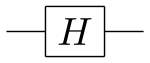
\includegraphics[width=0.3\textwidth]{img/hadamard.png}
  \caption{Schéma de circuit quantique pour la porte Hadamard (\cite{wikipediaPorteQuantique})}
\end{figure}

\textbf{Mesure} :
La mesure d'un qubit permet de lire son état. Elle est représentée par un symbole de balance dans
un schéma de circuit quantique. La mesure d'un qubit en superposition donne un résultat aléatoire
entre 0 et 1, avec une probabilité de 50\% pour chaque état. Elle prend dont un qubit en entrée et
renvoie un bit classique (0 ou 1) en sortie.

\textit{\textbf{Information :} Les deux lignes horizontales représentent un bit classique, tandis qu'une seule ligne représente un qubit.}

\begin{figure}[H]
  \centering
  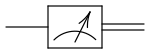
\includegraphics[width=0.3\textwidth]{img/mesure.png}
  \caption{Schéma de circuit quantique pour la mesure d'un qubit (\cite{wikipediaPorteQuantique})}
\end{figure}

\textbf{Circuit d'un algorithme de nombre aléatoire} :
Ce circuit quantique décris l'algorithme de génération de nombres aléatoires en informatique quantique. 

On travaille ici avec qu'un seul qubit \texttt{q} initialisé à l'état $\ket{0}$ ou $\ket{1}$ (conventionnellement, on choisit $\ket{0}$).
On applique ensuite une porte Hadamard à ce qubit pour le mettre dans un état de superposition. 
Enfin, on mesure le qubit pour obtenir un résultat aléatoire entre 0 et 1. 

Cette mesure est sortie dans la partie \texttt{c} du circuit (\texttt{c} signifie \textit{classique}).
Cette partie renvoie un bit classique, qui est le résultat de la mesure du qubit. En effet,
le \texttt{1} à droite de \texttt{c} signifie le nombre de bits classiques en sortie. Le \texttt{0}
à côté de la sortie de la mesure, signifie que le bit mesuré est à l'index numéro 0.


\begin{figure}[H]
  \centering
  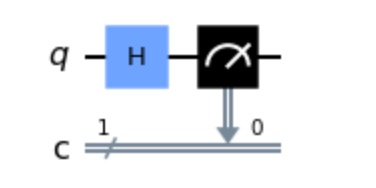
\includegraphics[width=0.5\textwidth]{img/portesLogiquesRandom.png}
  \caption{Portes logiques pour la génération d'un nombre aléatoire entre 0 et 1 (\cite{sapTrueRandomness})}
\end{figure}

\textbf{Circuit avec 8 qubits} :
Le problème avec le circuit précédent est qu'il ne génère qu'un seul bit aléatoire, ce qui veut dire que le nombre aléatoire généré est soit 0 soit 1. 
Pour générer un nombre aléatoire plus grand, il suffit de répéter le processus de préparation et de mesure de qubits en superposition plusieurs fois,
ou alors d'utiliser plusieurs qubits en superposition en même temps.

Ici, on obtient un circuit quantique pour la génération d'un nombre aléatoire avec 8 qubits.
En une seule exécution, ce circuit génère un nombre aléatoire entre 0 et 255 (car $2^8 = 256$).

\begin{figure}[H]
  \centering
  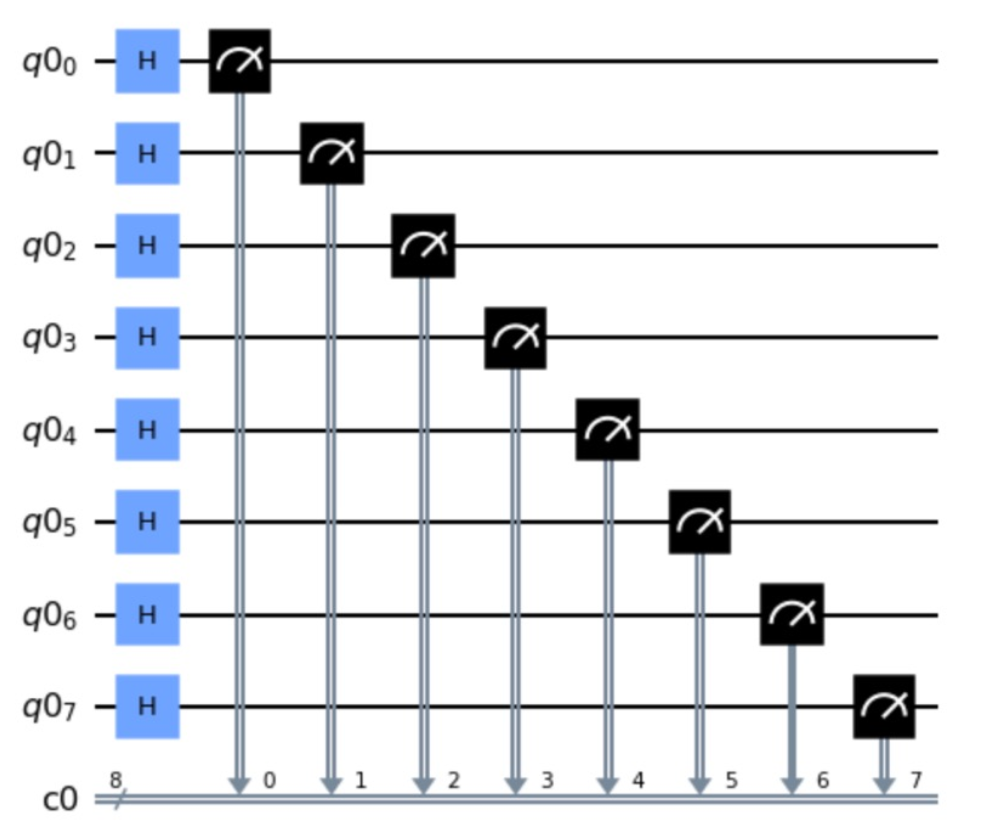
\includegraphics[width=0.7\textwidth]{img/portesLogiquesRandom8.png}
  \caption{Circuit quantique pour la génération d'un nombre aléatoire avec 8 qubits (\cite{sapTrueRandomness})}
\end{figure}

\subsection{Code de l'algorithme}

Dans cette partie, il est question de coder l'algorithme de génération de nombres aléatoires avec 8 qubits en informatique quantique en utilisant Qiskit.

\subsubsection{Prérequis}
Il est étonnament assez simple de coder un algorithme quantique en Python avec Qiskit. En voici les prérequis :

\begin{itemize}
  \item Installer Python : \texttt{https://www.python.org/downloads/}
  \item Installer Qiskit : \texttt{pip install qiskit}
  \item Installer Qiskit Aer : \texttt{pip install qiskit-aer} (\cite{qiskitGettingStarted})
\end{itemize}

Il est aussi préférable de coder sur Jupyter Notebook, qui permet d'exécuter du code Python en temps réel.

\subsubsection{Initialisation du circuit}

Le circuit quantique est initialisé avec 8 qubits en entrée et 8 bits classiques en sortie. On applique ensuite une porte Hadamard à chaque qubit pour les mettre dans un état de superposition, comme expliqué précédemment.
On mesure ensuite chaque qubit pour obtenir un résultat aléatoire entre 0 et 1, stocké dans leurs bits classiques respectifs. (Par exemple, le résultat du qubit 0 est stocké dans le bit classique 0, et ainsi de suite.)

\begin{lstlisting}[language=Python, style=mystyle, caption={Initialisation du circuit avec 8 qubits}]
  from qiskit import QuantumRegister, ClassicalRegister, QuantumCircuit, transpile
  from qiskit_aer import Aer
  
  q = QuantumRegister(8, 'q') # initialisation d'un registre quantique de 8 qubits
  c = ClassicalRegister(8, 'c') # initialisation d'un registre classique de 8 bits
  circuit = QuantumCircuit(q, c) # initialisation d'un circuit quantique avec les registres q et c
  
  circuit.h(q[0]) # porte de Hadamard sur le premier qubit
  circuit.h(q[1]) # porte de Hadamard sur le deuxieme qubit
  circuit.h(q[2]) # ...
  circuit.h(q[3])
  circuit.h(q[4])
  circuit.h(q[5])
  circuit.h(q[6])
  circuit.h(q[7])

  """ # simplification
  for elt_qubit in q:
      circuit.h(elt)
  """
  
  circuit.measure(q, c) # mesure de tous les qubits dans les bits classiques correspondants
\end{lstlisting}

\subsubsection{Exécution du circuit}

Pour exécuter le circuit, on utilise un simulateur quantique. Ici, on utilise le simulateur Aer de Qiskit, qui permet de simuler un ordinateur quantique sur un ordinateur classique.

À la fin de l'execution, on obtient en retour un dictionnaire contenant les résultats de la simulation, c'est-à-dire les nombres aléatoires générés.

\begin{lstlisting}[language=Python, style=mystyle, caption={Exécution du circuit}, label={lst:execution_circuit}]
  simulateur = Aer.get_backend('aer_simulator') # initialisation du simulateur Aer avec le backend aer_simulator
  circuitCompile = transpile(circuit, simulateur) # compilation du circuit pour le simulateur
  result = simulateur.run(circuitCompile, shots=1).result() # shot=1 veut dire qu'on execute le circuit une seule fois
  
  counts = result.get_counts(circuit)
  print("\nResultats de la mesure :", counts)  
\end{lstlisting}

\textit{\textbf{Note additionnelle} : On peut voir dans certains codes sur internet que le simulateur s'appelle \texttt{qasm\_simulator} au lieu de \texttt{aer\_simulator}. En effet, \texttt{qasm\_simulator} est une version nientôt obsolète du simulateur Aer. On conseille aujourd'hui d'utiliser \texttt{aer\_simulator} depuis peu. (\cite{stackexchangeWhatDifferences})}
\\ \\
En retour de cette exécution, on obtient un dictionnaire qui comporte le nombre binaire généré :
\begin{lstlisting}[style=mystyle, caption={Résultat de la mesure : \{'00001010': 1\}}]
  Resultats de la mesure : {'00001010': 1}
\end{lstlisting}
Ce dictionnaire contient le nombre binaire 8 bits généré, avec sa fréquence d'apparition. Il n'y a qu'une seule clé dans ce dictionnaire, qui est le nombre binaire généré, et la valeur associée est le nombre de fois que ce nombre a été généré (une seule fois car le circuit a été exécuté une fois, CF Listing \ref{lst:execution_circuit} \texttt{"shots=1"}).

Ici, le nombre généré est 00001010, qui correspond à 10 en décimal. On peut donc dire que le nombre aléatoire généré est 10.

\subsubsection{Visualisation du circuit}

Il est possible de visualiser le circuit quantique généré avec Qiskit. Pour cela, on utilise la méthode \texttt{circuit\_drawer()} du circuit.

\begin{lstlisting}[language=Python, style=mystyle, caption={Visualisation du circuit}]
  from qiskit import QuantumCircuit

  circuit_drawer(circuit, output='mpl')
\end{lstlisting}

On obtient bien un schéma de circuit quantique avec les portes Hadamard et les mesures, comme celle vue précédemment.

\begin{figure}[H]
  \centering
  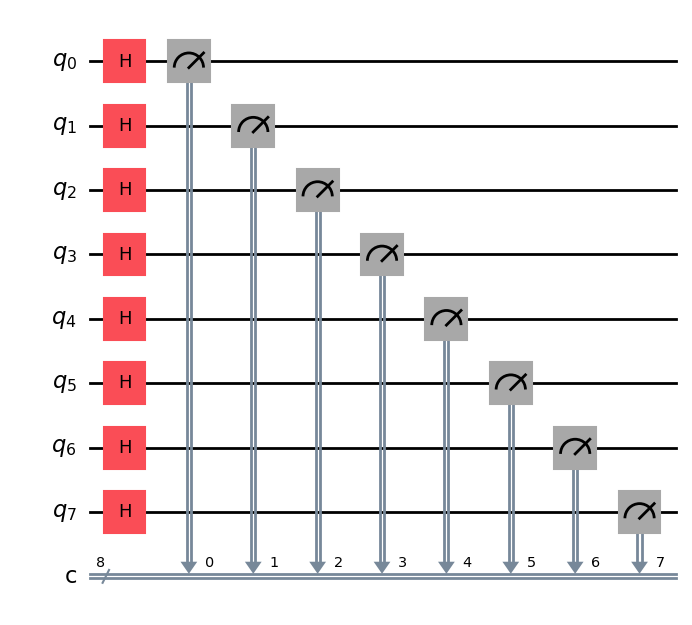
\includegraphics[width=0.7\textwidth]{img/circuitPy.png}
  \caption{Schéma de circuit quantique pour la génération d'un nombre aléatoire avec 8 qubits, généré à partir de Qiskit}
\end{figure}


\subsection{Conclusion de l'expérimentation}

Cette expérimentation est sûrement la plus simple à réaliser et à comprendre pour un débutant en informatique quantique. Elle permet de mettre en pratique les concepts de superposition et de mesure des qubits en quelques lignes de code.

Il n'y a pas grand chose à faire de plus si vous souhaitez essayer sur une vraie machine quantique, il suffit de changer le backend du simulateur Aer pour un vrai ordinateur quantique. Cependant, il est important de noter que les ordinateurs quantiques sont encore en développement et, il peut y avoir en conséquence, des erreurs dans les résultats.
Les simulations quantiques offrent une alternative plus fiable pour l'instant, bien qu'un manque de scalabilité soit présent pour des circuits plus complexes, ainsi qu'un manque de réalisme quantique.

\break\section{Limites et perspectives}

\subsection{Défis actuels}

Comme nous avons pu le voir, l’informatique quantique est une technologie prometteuse, offrant même l'espoir de voir l'humanité triompher de problèmes complexes. Mais elle reste confrontée à plusieurs défis majeurs qui ralentissent son développement et son adoption à grande échelle :  

\begin{enumerate}
  \item \textbf{Décohérence et correction d'erreurs} \\
  L’un des problèmes les plus importants est la décohérence quantique, qui entraîne une perte rapide d’information lorsque les qubits interagissent et sont perturbés par leur environnement. Cela limite le temps de calcul utile et nécessite des techniques avancées de correction d'erreurs quantiques. Cependant, les codes correcteurs actuels nécessitent des dizaines, voire des centaines de qubits physiques (qui ne sont pas utilisés directement pour le calcul) pour stabiliser un seul qubit logique (utilisé pour le calcul). Nous verrons que de récentes avancées ont été réalisées sur ce sujet. 

  \item \textbf{Scalabilité et fiabilité des qubits} \\
  La mise à l’échelle des ordinateurs quantiques est un autre défi. Les processeurs quantiques actuels possèdent encore un nombre limité de qubits exploitables. Par exemple, IBM et Google ont construit des processeurs atteignant respectivement 1125* et 105 qubits physiques qui sont encore loin des milliers de qubits stables nécessaires pour des calculs pratiques. (*il est important de noter que la qualité des qubits (comment ils sont gérés, mesurés) est aussi, voir plus importante que leur quantité pour le moment. Tous les qubits de se valent pas !)  

  \item \textbf{Puissance de calcul réelle vs promesses théoriques} \\
  Si des algorithmes comme celui de (\cite{wikipediaAlgorithmeShor}) pour la factorisation ou de Grover pour la recherche dans une base de données sont souvent mis en avant, les gains quantiques restent difficiles à exploiter sur les machines actuelles. Les résultats restent contestés et encore loin d’une application industrielle généralisée. 

  \item \textbf{Besoin en infrastructure cryogénique} \\
  La plupart des technologies de qubits nécessitent un refroidissement à des températures proches du zéro absolu (~15 mK), ce qui augmente les coûts et rend difficile leur intégration dans des systèmes informatiques conventionnels. 
\end{enumerate}

\subsection{Futur de l'informatique quantique}

Malgré ces défis, l’informatique quantique continue de progresser rapidement, avec plusieurs avancées notables qui pourraient accélérer son adoption. 

\begin{enumerate}
  \item \textbf{L’essor des qubits topologiques} \\
  Microsoft travaille activement sur des qubits topologiques, plus résistants aux perturbations et aux erreurs. En 2025, l'entreprise a annoncé avoir réussi à présenter le Majorana 1, une puce quantique utilisant des qubits topologiques fabriqués à partir de nouveaux matériaux, les topoconducteurs. Un état de la matière qui ouvre la voie à des qubits plus stables et plus performants. Cette avancée pourrait permettre de construire des ordinateurs quantiques dotés de millions de qubits dans un avenir proche, offrant ainsi une fiabilité accrue pour des applications de calculs quantiques à grande échelle. \cite{microsoftMajorana}

  \item \textbf{Hybrides quantique-classique} \\
  Une approche prometteuse consiste à coupler des algorithmes quantiques à des processeurs classiques. Des entreprises comme NVIDIA et Amazon développent des plateformes hybrides permettant d’utiliser des circuits quantiques comme accélérateurs spécialisés pour l’optimisation et l’apprentissage automatique. 

  \item \textbf{Applications concrètes en développement} \\
  Bien que la cryptographie post-quantique soit un domaine majeur, d'autres secteurs comme la chimie (modélisation de molécules complexes), la finance (optimisation de portefeuilles), et la logistique (optimisation de trajets) commencent à expérimenter des solutions hybrides incluant du calcul quantique. 

  \item \textbf{Démocratisation via le cloud} \\
  L’accès aux ordinateurs quantiques via le cloud (IBM Quantum, Azure Quantum, AWS Braket) permet à de plus en plus de chercheurs et d'entreprises d’expérimenter et d’optimiser des algorithmes quantiques, facilitant ainsi l'émergence d'applications pratiques. 
\end{enumerate}

Si les défis rencontrés la peuvent sembler inquiétant, ces avancés permettent d'apercevoir un futur brillant pour cette discipline. Il faut aussi se rappeler que nous faisions face à des problèmes similaires aux débuts de l’informatique classique :  

Les premiers ordinateurs classiques comme l'ENIAC (1945) étaient lents, énergivores et peu fiables. Leur évolution a nécessité des décennies pour atteindre des machines plus rapides et fiables, comme les premiers processeurs à transistors. 

\begin{table}[H]
\centering
\begin{tabular}{|l|l|}
  \hline
  \textbf{Premiers “processeurs” classiques} & \textbf{Processeurs modernes (i9)} \\
  \hline
  100 kHz & 5,2 GHz (52 000x supérieur) \\
  \hline
\end{tabular}
\caption{Évolution des processeurs classiques}
\end{table}

De même, l’informatique quantique aujourd'hui est limitée par des qubits fragiles, soumis à la décohérence et au bruit. Mais nous pouvons observer les mêmes avancées majeures qu’il y a 60 ans : 

\begin{table}[H]
\centering
\begin{tabular}{|l|l|l|l|}
  \hline
  \textbf{Processeurs} & \textbf{Année} & \textbf{Qubits} & \textbf{Quantique vs Classique} \\
  \hline
  Sycamore (Google) & 2019 & 70 & $10^4$ ans -> 200 secondes \\
  Willow (Google) & 2024 & 105 & $10^{25}$ ans -> 5 min \\
  \hline
\end{tabular}
\caption{Évolution des processeurs quantiques}
\end{table}

\cite{googleWillow} \cite{wikipediaSycamore} \cite{wikipediaQProcessors}

\break\section{Conclusion et Q\&A}
\subsection{Récapitulatif des points clés}
\begin{itemize}
  \item L'informatique quantique utilise les principes de la mécanique quantique pour effectuer des calculs.
  \item Les qubits sont la base de l'informatique quantique, permettant la superposition et l'intrication.
  \item Les portes quantiques manipulent les qubits pour effectuer des opérations logiques.
  \item La mesure d'un qubit en superposition donne un résultat aléatoire, permettant la génération de nombres aléatoires.
  \item L'informatique quantique est confrontée à des défis majeurs, mais des avancées prometteuses sont en cours.
  \item L'informatique quantique a le potentiel de révolutionner des domaines tels que la cryptographie, l'optimisation et la simulation de systèmes quantiques.
  \item Des entreprises comme IBM, Google et Microsoft investissent massivement dans la recherche et le développement de l'informatique quantique.
\end{itemize}

\subsection{Session de questions-réponses}

\begin{itemize}
  \item \textbf{Q1: Quelle est la différence entre un ordinateur quantique et un simulateur quantique?}
  \item Réponse: Un ordinateur quantique utilise des qubits physiques pour effectuer des calculs basés sur la mécanique quantique, tandis qu'un simulateur quantique utilise un ordinateur classique pour imiter le comportement d'un ordinateur quantique. Les simulateurs sont utiles pour le développement et le test d'algorithmes quantiques, mais ils ne peuvent pas reproduire pleinement les avantages de la véritable computation quantique.

  \item \textbf{Q2: Quels sont les principaux langages de programmation utilisés pour développer des algorithmes quantiques?}
  \item Réponse: Les principaux langages de programmation pour les algorithmes quantiques incluent Qiskit (Python) développé par IBM, Cirq (Python) développé par Google, et Q\# développé par Microsoft.

  \item \textbf{Q3: Comment les ordinateurs quantiques peuvent-ils améliorer la cryptographie?}
  \item Réponse: Les ordinateurs quantiques peuvent briser les systèmes de cryptographie actuels basés sur la factorisation de grands nombres (comme RSA) en utilisant des algorithmes comme celui de Shor (\cite{wikipediaAlgorithmeShor}). Ils peuvent également renforcer la cryptographie en permettant la création de clés de chiffrement véritablement aléatoires et en facilitant la mise en œuvre de la cryptographie quantique.

  \item \textbf{Q4: Quels sont les défis liés à la correction d'erreurs dans les ordinateurs quantiques?}
  \item Réponse: La correction d'erreurs quantiques est un défi majeur en raison de la sensibilité des qubits à leur environnement, ce qui peut entraîner des erreurs de décohérence et de bruit. Les codes de correction d'erreurs quantiques nécessitent un grand nombre de qubits physiques pour protéger un seul qubit logique.

  \item \textbf{Q5: Comment les ordinateurs quantiques peuvent-ils être utilisés dans l'optimisation?}
  \item Réponse: Les ordinateurs quantiques peuvent résoudre des problèmes d'optimisation complexes plus efficacement que les ordinateurs classiques en utilisant des algorithmes quantiques comme l'algorithme de Grover (\cite{wikipediaAlgorithmeGrover}). Par exemple, pour trouver un élément dans une liste de $n$ éléments, un algorithme classique a une complexité de $O(n)$, tandis qu'un algorithme quantique a une complexité de $O(\sqrt{n})$, ce qui est beaucoup plus rapide.
  
  \item \textbf{Q6: Quels sont les principaux obstacles à l'adoption généralisée des ordinateurs quantiques?}
  \item Réponse: Les principaux obstacles incluent la décohérence, le bruit des qubits, la mise à l'échelle des systèmes, le besoin en infrastructure cryogénique, et le développement de logiciels et d'algorithmes adaptés. De plus, il est nécessaire de former des experts en informatique quantique.
  
  \item \textbf{Q7: Qu'avez-vous appris de cette présentation?}
  \item Réponse: Nous nous intéressions déjà pas mal à l'informatique quantique, mais cela nous a permis de mieux comprendre les concepts de base suivant les mathématiques et la physique quantique. Coder un algorithme quantique était une première pour nous.
  
  \item \textbf{Q8: Que pensez-vous de l'informatique quantique?}
  \item Réponse: Ce sujet nous fait comprendre assez rapidement que nous vivons encore aux touts débuts de l'informatique quantique et qu'il nécessite encore beaucoup de recherche et de développement pour exploiter pleinement son potentiel. Cependant, nous sommes très enthousiastes à l'idée de voir comment cette technologie va évoluer dans les années à venir et comment elle pourrait transformer notre façon de traiter l'information.
\end{itemize}

\break\section{Annexes}
\subsection{Glossaire}
\begin{itemize}
  \item \textbf{Algorithme de Grover} : Algorithme quantique pour la recherche dans une base de données non structurée. (\cite{wikipediaAlgorithmeGrover})
  \item \textbf{Algorithme de Shor} : Algorithme quantique pour la factorisation de grands nombres, qui menace la cryptographie classique. (\cite{wikipediaAlgorithmeShor})
  \item \textbf{Cirq} : Framework open-source développé par Google pour la programmation d'algorithmes quantiques.
  \item \textbf{Correction d'erreurs quantiques} : Techniques utilisées pour protéger les qubits contre les erreurs causées par la décohérence et le bruit.
  \item \textbf{Décohérence} : Perte d'information quantique due à l'interaction avec l'environnement.
  \item \textbf{IBM Quantum Experience} : Plateforme cloud d'IBM permettant d'accéder à des ordinateurs quantiques.
  \item \textbf{Intrication} : Propriété quantique où deux qubits sont liés de telle manière que l'état de l'un dépend de l'état de l'autre.
  \item \textbf{Mesure} : Processus d'obtention d'un résultat classique à partir d'un qubit en superposition.
  \item \textbf{Porte quantique} : Opération qui agit sur un ou plusieurs qubits pour effectuer des calculs.
  \item \textbf{Q\#} : Langage de programmation quantique développé par Microsoft.
  \item \textbf{QASM} : Quantum Assembly Language, un langage de bas niveau pour représenter des circuits quantiques.
  \item \textbf{Qiskit} : Framework open-source pour la programmation d'algorithmes quantiques en Python.
  \item \textbf{Qubit} : Unité de base de l'information quantique, analogue au bit classique.
  \item \textbf{Superposition} : État dans lequel un qubit peut représenter simultanément plusieurs valeurs.
  \item \textbf{Topoconducteurs} : Matériaux utilisés pour fabriquer des qubits topologiques, offrant une meilleure stabilité et performance.
\end{itemize}

\subsection{Liens utiles}
\begin{itemize}
  \item \textbf{Cirq} : \url{https://quantumai.google/cirq}
  \item \textbf{Google Quantum AI} : \url{https://quantumai.google/}
  \item \textbf{IBM Quantum Experience} : \url{https://quantum-computing.ibm.com/}
  \item \textbf{Microsoft Quantum Development Kit} : \url{https://azure.microsoft.com/en-us/services/quantum-development-kit/}
  \item \textbf{Q\#} : \url{https://docs.microsoft.com/en-us/quantum/}
  \item \textbf{QASM} : \url{https://www.quantum-inspire.com/kbase/cqasm/}
  \item \textbf{Qiskit} : \url{https://qiskit.org/}
  \item \textbf{Stack Exchange} : \url{https://quantumcomputing.stackexchange.com/}
  \item \textbf{Wikipedia} : \url{https://fr.wikipedia.org/wiki/Informatique_quantique}
\end{itemize}

\subsection{L'utilisation de l'intelligence artificielle pour la recherche et la rédaction}

L'intelligence artificielle peut se sembler extrêmement utile pour obtenir des informations assez précises sur certains domaines de ce sujet.

Nous avons en effet utiliser l'intelligence artificielle pour, par exemple, avoir la confirmation du fait qu'un un simulateur quantique utilisait bien un algorithme pseudo-aléatoire pour simuler la mesure d'un qubit.

Voici quelques une des questions posées à l'IA :

\begin{itemize}
  \item \textit{Comment un simulateur quantique arrive à creer des qubits/porte d'Hadamarde ?}
  \item \textit{Dans cet exemple (expliqué plus tôt par l'IA), comment mesure-t-on ce qubit ?}
  \item \textit{Si l'on fixe une seed, et que l'on a trois qubits initialisés à 0 et un initialisé à 1. Est-ce qu'apres la porte d'Hadamarde, le bit initialisé à 1 sera forcément different de ceux à 0 suite à la mesure ? (toujours dans un cadre de simulation) }
  \item \textit{À quel point l'enjeu d'avoir un ordinateur quantique est important dans la création d'un nombre purement aléatoire ? Recherche, si jamais, des interview, etc... }
  \item \textit{Existe-t-il d'autres domaines qui nécessitent d'autant plus les ordinateurs quantique ?}
\end{itemize}

La recherche par image a aussi été utilisée pour obtenir une description et explication plus détaillée sur les circuits quantiques

\medskip

Sur le contenu de ce rapport, l'IA a pu juger de la pertinence de certaines phrases, et de la formulation de celles-ci. Nous doutions aussi du fait que nous parlions un peu trop de la physique quantique et pas assez de l'algorithme quantique, l'IA a pu nous suggérer des changements de contenus pour rééquilibrer le rapport.

\medskip

Nous avons aussi pu utiliser l'IA pour rallonger certains paragraphes, en lui demandant de reformuler certaines phrases, ou de les développer.

L'IA a permis de corriger certaines fautes d'orthographes, de certains problèmes de compilation en Latex, et de nous aider à écrire certaines équations.

L'aide à la mise en page a aussi été très utile, en nous suggérant de mettre certaines parties en gras, ou d'ajouter des titres pour mieux structurer le rapport.


\break\section{Bibliographie}
\printbibliography

\end{document}